\documentclass[11pt,letterpaper]{article}
\usepackage[margin=1in]{geometry}
\usepackage{graphicx}
\usepackage{booktabs}
\usepackage{multirow}
\usepackage{xcolor}
\usepackage{colortbl}
\usepackage{hyperref}
\usepackage{float}
\usepackage{caption}
\usepackage{subcaption}
\usepackage{enumitem}
\usepackage{amsmath}
\usepackage{tabularx}
\usepackage{array}

\definecolor{toprow}{HTML}{E8F5E9}
\definecolor{midrow}{HTML}{FFF3E0}
\definecolor{botrow}{HTML}{FFEBEE}
\definecolor{zerorow}{HTML}{F5F5F5}
\definecolor{sectionblue}{HTML}{1565C0}

\hypersetup{
  colorlinks=true,
  linkcolor=sectionblue,
  urlcolor=sectionblue,
  citecolor=sectionblue
}

\newcommand{\smark}[1]{\textcolor{gray}{\scriptsize #1}}

\title{\textbf{LENS Benchmark: Project Brief}\\[0.3em]
\large Longitudinal Evidence-backed Narrative Signals\\[0.2em]
\normalsize Evaluating Agent Memory Systems for Multi-Episode Synthesis}
\author{Project Status Report --- March 2026}
\date{}

\begin{document}
\maketitle
\thispagestyle{empty}

\begin{abstract}
\noindent
LENS is a benchmark that tests whether AI agent memory systems can synthesize conclusions from evidence scattered across many sequential episodes. Over 28 sessions spanning February--March 2026, we evaluated 8 memory architectures across 9 domain-diverse scopes (6~numeric, 3~narrative), totaling 150+ scored benchmark runs. The central finding is a negative result: \textbf{no dedicated memory architecture outperforms a simple SQLite-backed hybrid retrieval baseline} (chunked embeddings + FTS5 keyword search + reciprocal rank fusion). All architectures that preprocess evidence---summarization, entity extraction, graph construction, memory consolidation---destroy the fine-grained detail that longitudinal synthesis requires. The benchmark's core challenge (composite scores capped at~0.50) remains unsolved, suggesting fundamental limitations in current retrieval-augmented generation approaches to multi-episode reasoning.
\end{abstract}

\tableofcontents
\newpage

%% ============================================================
\section{Introduction}
%% ============================================================

The AI memory ecosystem in 2025--2026 produced a wave of agent memory systems---Mem0, Letta (formerly MemGPT), Graphiti, Cognee, Hindsight, and others---each claiming to provide persistent, queryable memory for LLM agents. These systems promise to solve the ``goldfish problem'': LLMs forget everything between conversations.

But do they actually help agents \emph{reason} across long sequences of information? LENS answers this question with a benchmark designed around a specific cognitive challenge: \textbf{longitudinal synthesis}---assembling fragments of evidence from dozens of separate observations to reach a conclusion that no single observation supports.

\subsection{What LENS Tests}

Each LENS scope presents an agent with 20--120 sequential episodes (simulated system logs, clinical reports, financial filings, chat transcripts, or corporate documents). Hidden within these episodes is a slowly developing signal: a cascading infrastructure failure, a clinical drug interaction, a shadow API attack. Critically:

\begin{itemize}[nosep]
  \item No single episode contains enough information to answer any benchmark question
  \item Signal is encoded as numeric progressions (latency values, drug levels, request counts), not prose commentary
  \item 60--75\% of episodes are format-matched \emph{distractors}---topically orthogonal content that matches the format but is about entirely different subjects
\end{itemize}

The agent uses a memory system to ingest episodes, then answers 10--12 questions per checkpoint under a fixed token budget. Success requires the memory system to preserve fine-grained evidence while enabling efficient retrieval across a growing corpus.

\subsection{Project Scope}

\begin{itemize}[nosep]
  \item \textbf{28 sessions} over 14 days (Feb 16 -- Mar 1, 2026)
  \item \textbf{9 scopes}: 6 numeric/structured + 3 narrative/natural-language
  \item \textbf{8 adapters} in final evaluation (+ 2 disqualified)
  \item \textbf{150+ scored runs} with 3-tier composite scoring
  \item \textbf{992 unit tests} passing
  \item \textbf{Infrastructure}: Modal (H100 vLLM + T4 embeddings), Podman containers for Letta/FalkorDB/Qdrant
\end{itemize}

%% ============================================================
\section{Methodology}
%% ============================================================

\subsection{Dataset Generation: Information Isolation}

The most critical methodological decision addresses \textbf{LLM contamination}: when a single model generates benchmark episodes knowing the storyline, it editorializes. Instead of writing \texttt{p99: 600ms}, it writes ``latency is concerning''---making every episode a standalone causal analysis that answers all questions. This renders the benchmark worthless.

The solution is a \textbf{two-stage progressive expansion} with strict information isolation:

\begin{enumerate}[nosep]
  \item \textbf{PlanOutline} (GPT-5.2, sees full spec): Produces per-episode structured data sheets with concrete metric values. Signal encoded as numeric progressions only.
  \item \textbf{RenderEpisodes} (GPT-4.1-nano, blind to storyline): Formats each data sheet into a terse log entry independently. Cannot editorialize because it does not know what constitutes signal.
\end{enumerate}

Quality gates enforced by the pipeline: contamination (max single-episode question coverage) $<80\%$, naive baseline $<50\%$, forbidden words $= 0$.

\subsection{Adapter Interface}

All memory systems conform to a common \texttt{MemoryAdapter} interface:

\begin{itemize}[nosep]
  \item \texttt{ingest(episode)} --- store an episode (timeline phase, no budget clock)
  \item \texttt{prepare()} --- optional pre-processing before the question-answering phase
  \item \texttt{search(query)} / \texttt{batch\_retrieve(ref\_ids)} --- retrieve during budget-metered Q\&A
  \item \texttt{reset()} --- clean state between scopes
\end{itemize}

Key design insight: \textbf{LLM processing belongs in \texttt{prepare()}, not \texttt{ingest()}}. Adapters that process during \texttt{prepare()} achieve perfect budget compliance; those that process during the metered phase suffer catastrophic budget violations.

\subsection{Three-Tier Scoring (v3.2)}

\begin{table}[H]
\centering
\small
\begin{tabular}{llll}
\toprule
\textbf{Tier} & \textbf{Metrics} & \textbf{Method} & \textbf{Weight} \\
\midrule
1 (Mechanical) & evidence\_grounding, fact\_recall, & Exact computation & 40\% \\
               & evidence\_coverage, budget\_compliance, & & \\
               & citation\_coverage & & \\
\addlinespace
2 (LLM Judge)  & answer\_quality, insight\_depth, & Pairwise A/B judging & 40\% \\
               & reasoning\_quality & with position debiasing & \\
\addlinespace
3 (Differential) & naive\_baseline\_advantage, & Head-to-head vs & 20\% \\
                 & action\_quality & context-stuffed answer & \\
\bottomrule
\end{tabular}
\caption{Scoring tiers. Hard gate: \texttt{evidence\_grounding} $\geq 0.5$ or composite $= 0$.}
\label{tab:scoring}
\end{table}

The Tier~3 \emph{naive baseline advantage} is the most informative metric: does the memory-augmented answer beat what you get by simply stuffing all episodes into the context window? A score $>0.5$ means the memory system adds value; $<0.5$ means it harms.

%% ============================================================
\section{Adapters Evaluated}
%% ============================================================

\begin{table}[H]
\centering
\small
\begin{tabularx}{\textwidth}{lXl}
\toprule
\textbf{Adapter} & \textbf{Architecture} & \textbf{Status} \\
\midrule
\textbf{null} & No memory. Establishes absolute floor. & Baseline \\
\textbf{sqlite-chunked-hybrid} & Section-chunked embeddings + FTS5 + RRF + batch\_retrieve. Zero external deps. & \cellcolor{toprow}Top performer \\
\textbf{compaction} & Summarize-then-answer: re-summarize all episodes at each checkpoint. & Collapsed w/ distractors \\
\textbf{mem0-raw} & Pure vector search (Mem0 with extraction disabled). Qdrant backend. & Mid-tier \\
\textbf{letta} & Semantic vector search over archival passages. Podman + embed proxy. & Mid-tier \\
\textbf{letta-sleepy} & Letta + LLM sleep consolidation (delta/causal framing). & Mid-tier \\
\textbf{cognee} & Embedded GraphRAG (LanceDB + Kuzu + SQLite). No container. & 2nd place \\
\textbf{graphiti} & Temporal knowledge graph (FalkorDB, bi-temporal edges). & 3rd (incomplete) \\
\addlinespace
\textit{mem0-extract} & Mem0 with extraction enabled. & \cellcolor{botrow}Disqualified (0.000) \\
\textit{hindsight} & TEMPR multi-network (vectorize.io). & \cellcolor{botrow}Removed (= null) \\
\bottomrule
\end{tabularx}
\caption{All adapters evaluated. Mem0-extract disqualified (hardcoded ``Personal Information Organizer'' prompt returns zero facts from structured data). Hindsight removed (NBA statistically indistinguishable from null, 17.3\,GB image, 19/24 budget violations).}
\label{tab:adapters}
\end{table}

%% ============================================================
\section{Phase 5: Numeric Scope Results}
\label{sec:phase5}
%% ============================================================

Phase~5 is the definitive evaluation: 8 adapters $\times$ 6 scopes $\times$ 2 budgets (8k/16k tokens) with 120-episode distractor datasets. Agent LLM: GPT-OSS-120B (Cerebras). 90 of 96 runs scored (Graphiti timed out on 3 scopes).

\subsection{Overall Rankings}

\begin{table}[H]
\centering
\small
\begin{tabular}{rlccccc}
\toprule
\textbf{Rank} & \textbf{Adapter} & \textbf{8k Mean} & \textbf{95\% CI} & \textbf{16k Mean} & \textbf{$\Delta$} & \textbf{N} \\
\midrule
\rowcolor{toprow}
1 & sqlite-chunked-hybrid & 0.454 & [0.406, 0.502] & 0.492 & +8.2\% & 12/12 \\
\rowcolor{toprow}
2 & cognee & 0.421 & [0.397, 0.446] & 0.444 & +5.4\% & 12/12 \\
3 & graphiti & 0.393 & [0.220, 0.491] & 0.459 & +17.0\% & 6/12 \\
4 & mem0-raw & 0.330 & [0.265, 0.388] & 0.368 & +11.8\% & 12/12 \\
5 & letta & 0.327 & [0.258, 0.399] & 0.368 & +12.8\% & 12/12 \\
6 & letta-sleepy & 0.322 & [0.268, 0.381] & 0.360 & +11.7\% & 12/12 \\
7 & compaction & 0.245 & [0.137, 0.328] & 0.300 & +22.5\% & 12/12 \\
\rowcolor{zerorow}
8 & null & 0.000 & [0.000, 0.000] & 0.000 & --- & 12/12 \\
\bottomrule
\end{tabular}
\caption{Phase~5 composite scores. Bootstrap 95\% CIs (1000 resamples, 6 scopes). Kendall's $W = 0.755$ (strong cross-scope concordance). 16k $>$ 8k for all adapters ($p = 0.016$, Wilcoxon).}
\label{tab:phase5-rankings}
\end{table}

\begin{figure}[H]
\centering
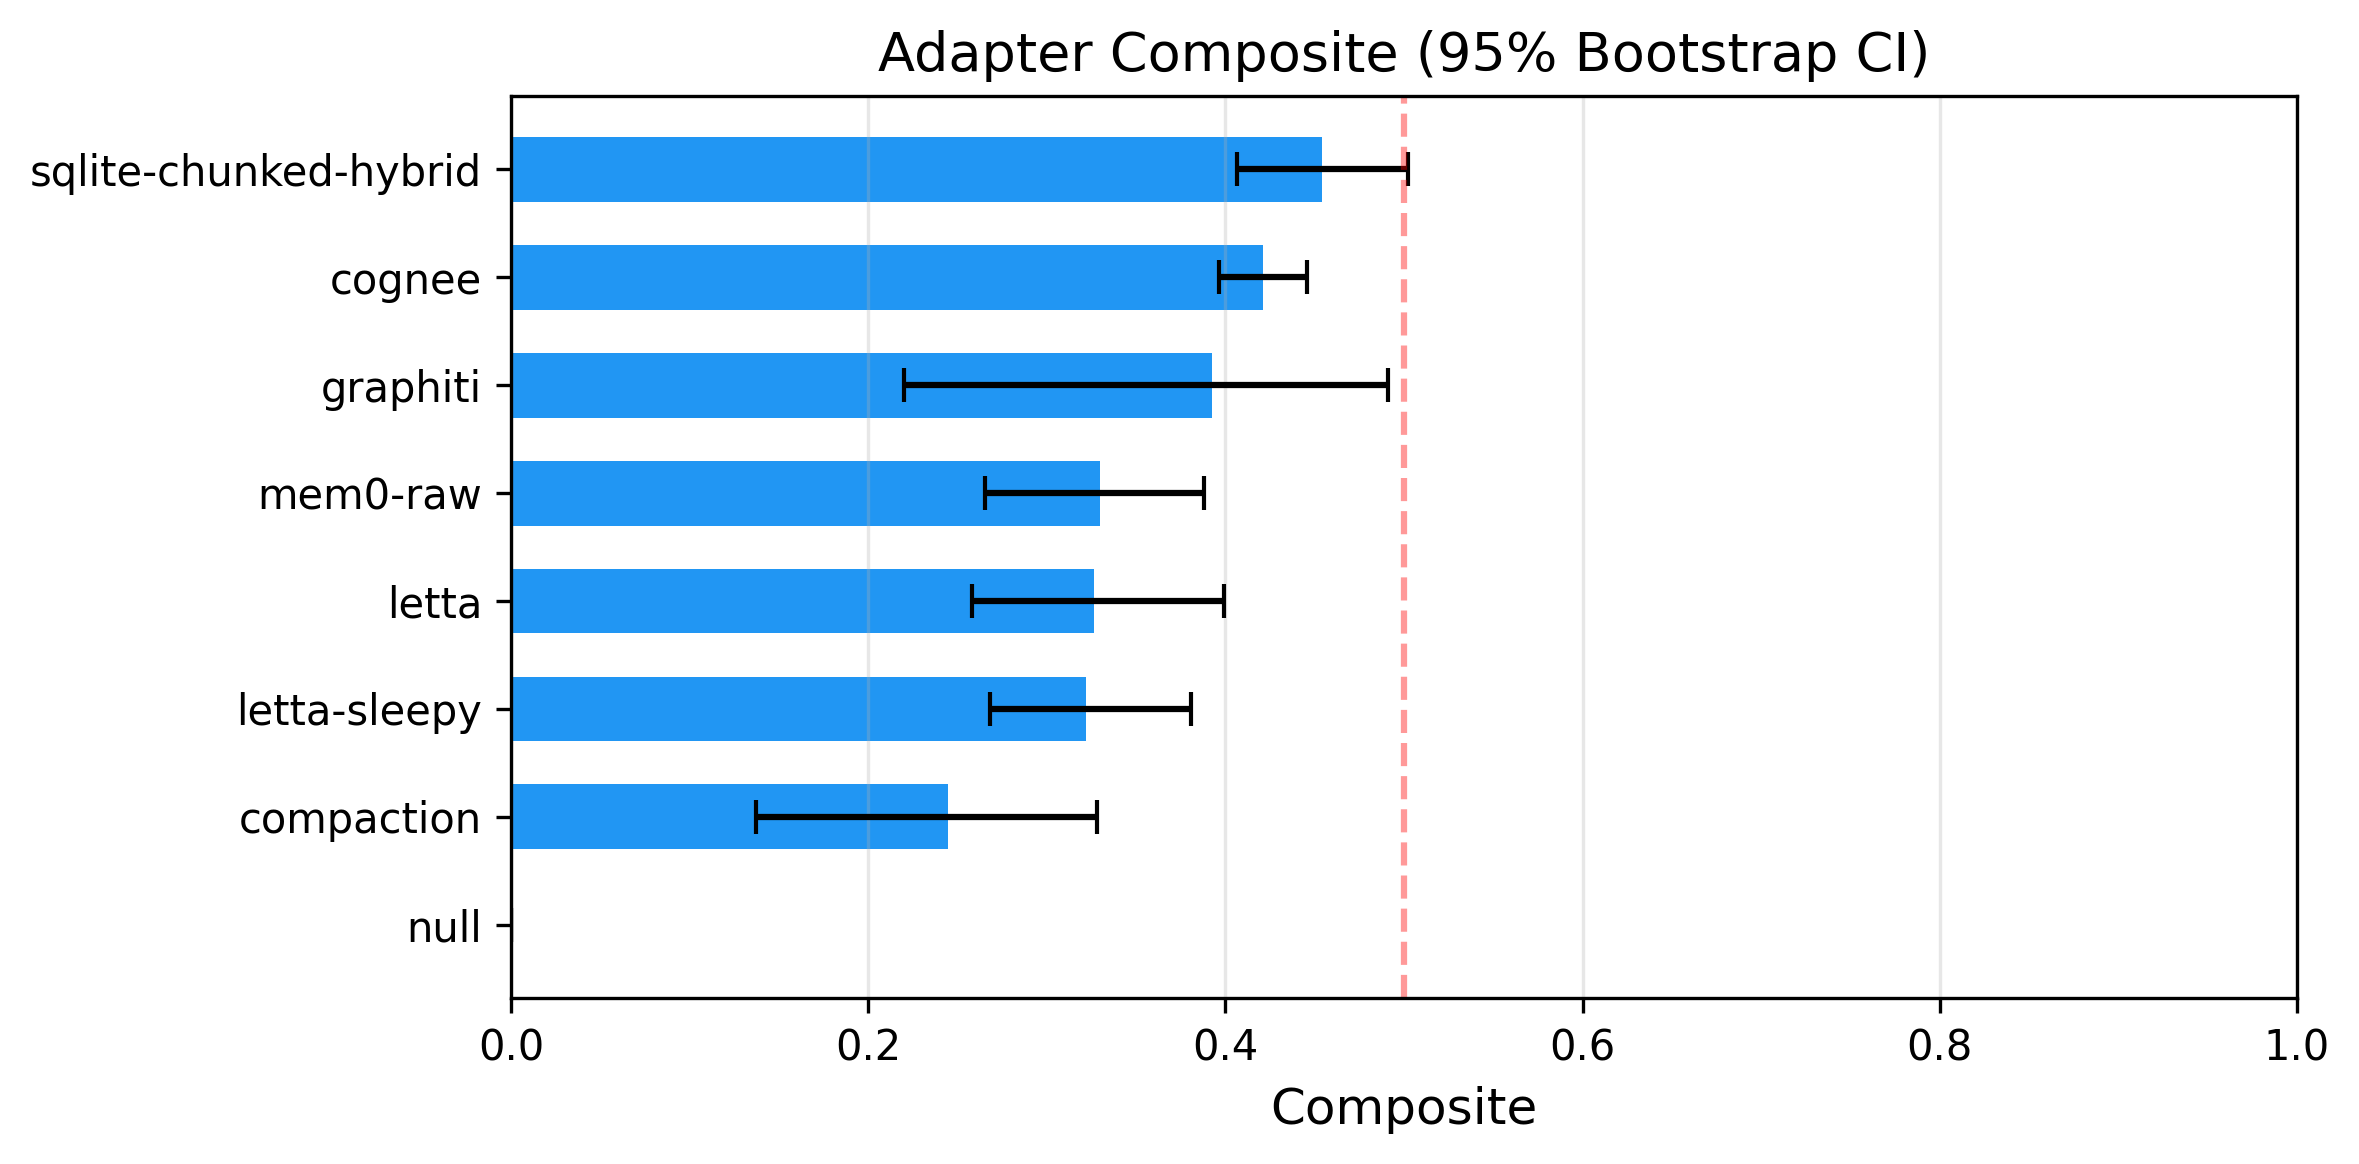
\includegraphics[width=0.85\textwidth]{figures/d1_answer_quality_ci.png}
\caption{Answer quality with 95\% confidence intervals across 6 numeric scopes.}
\label{fig:answer-quality}
\end{figure}

\subsection{Cross-Scope Consistency}

\begin{figure}[H]
\centering
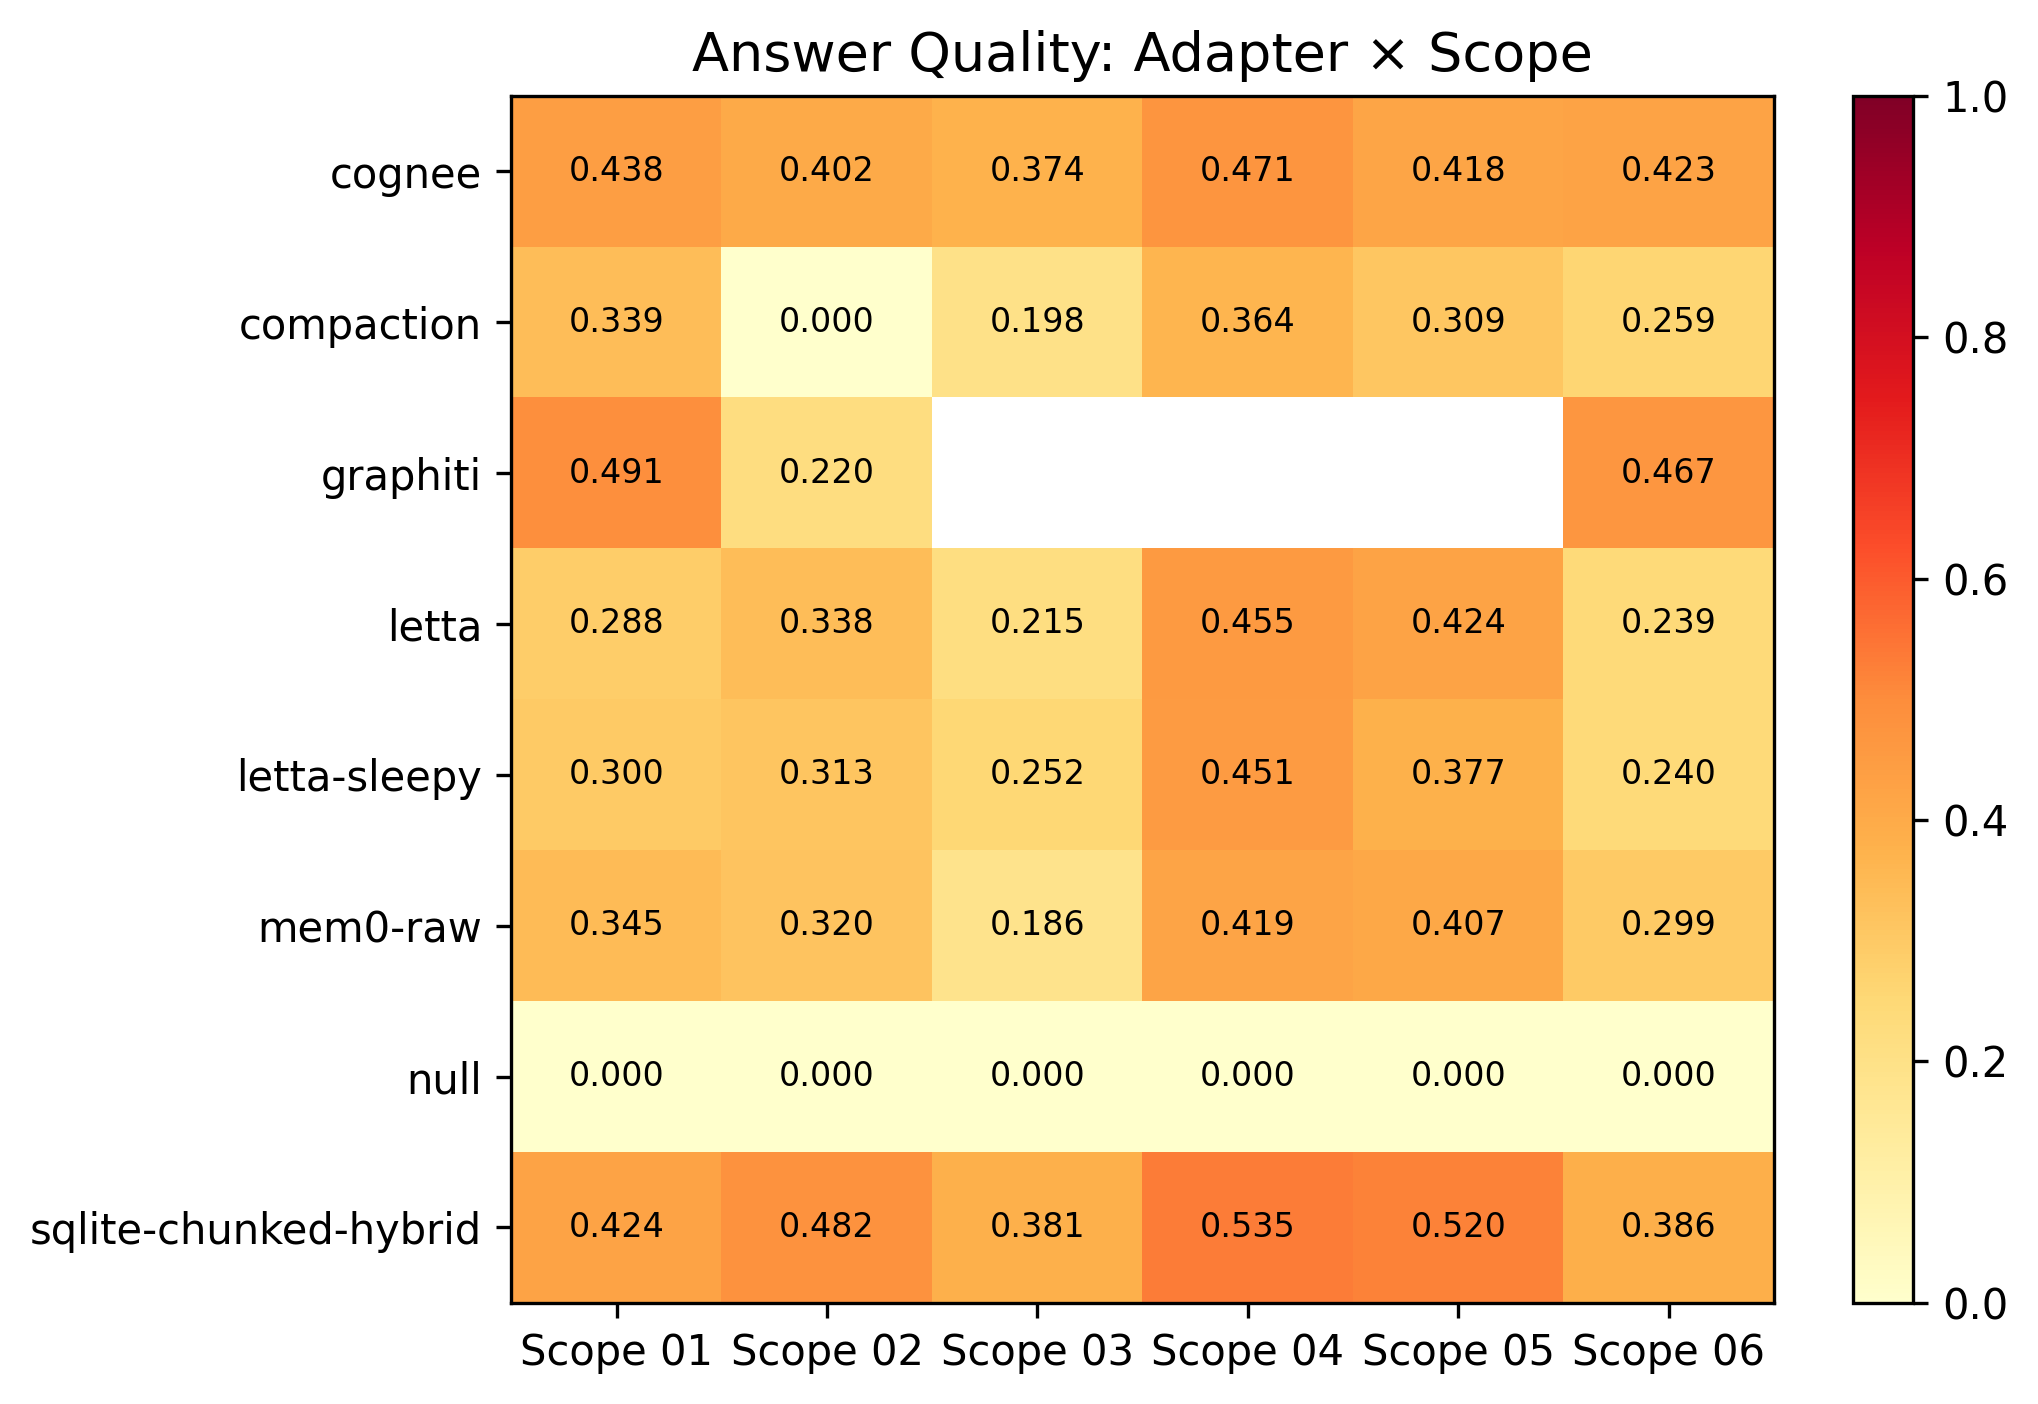
\includegraphics[width=0.85\textwidth]{figures/d2_heatmap.png}
\caption{Adapter $\times$ scope composite heatmap (8k budget). Rankings remain broadly stable across domains (Kendall's $W = 0.755$), but scope difficulty varies: S04 (cloud outage) is easiest; S03 (clinical signals) is hardest.}
\label{fig:heatmap}
\end{figure}

\subsection{Budget Scaling}

All adapters benefit from 16k vs 8k budgets (mean $+12\%$), but none achieve budget compliance---every adapter exceeds the cumulative token limit on the first retrieval call. The budget enforcement mechanism cannot ``un-retrieve'' an already-oversized first result.

\begin{figure}[H]
\centering
\begin{subfigure}[t]{0.48\textwidth}
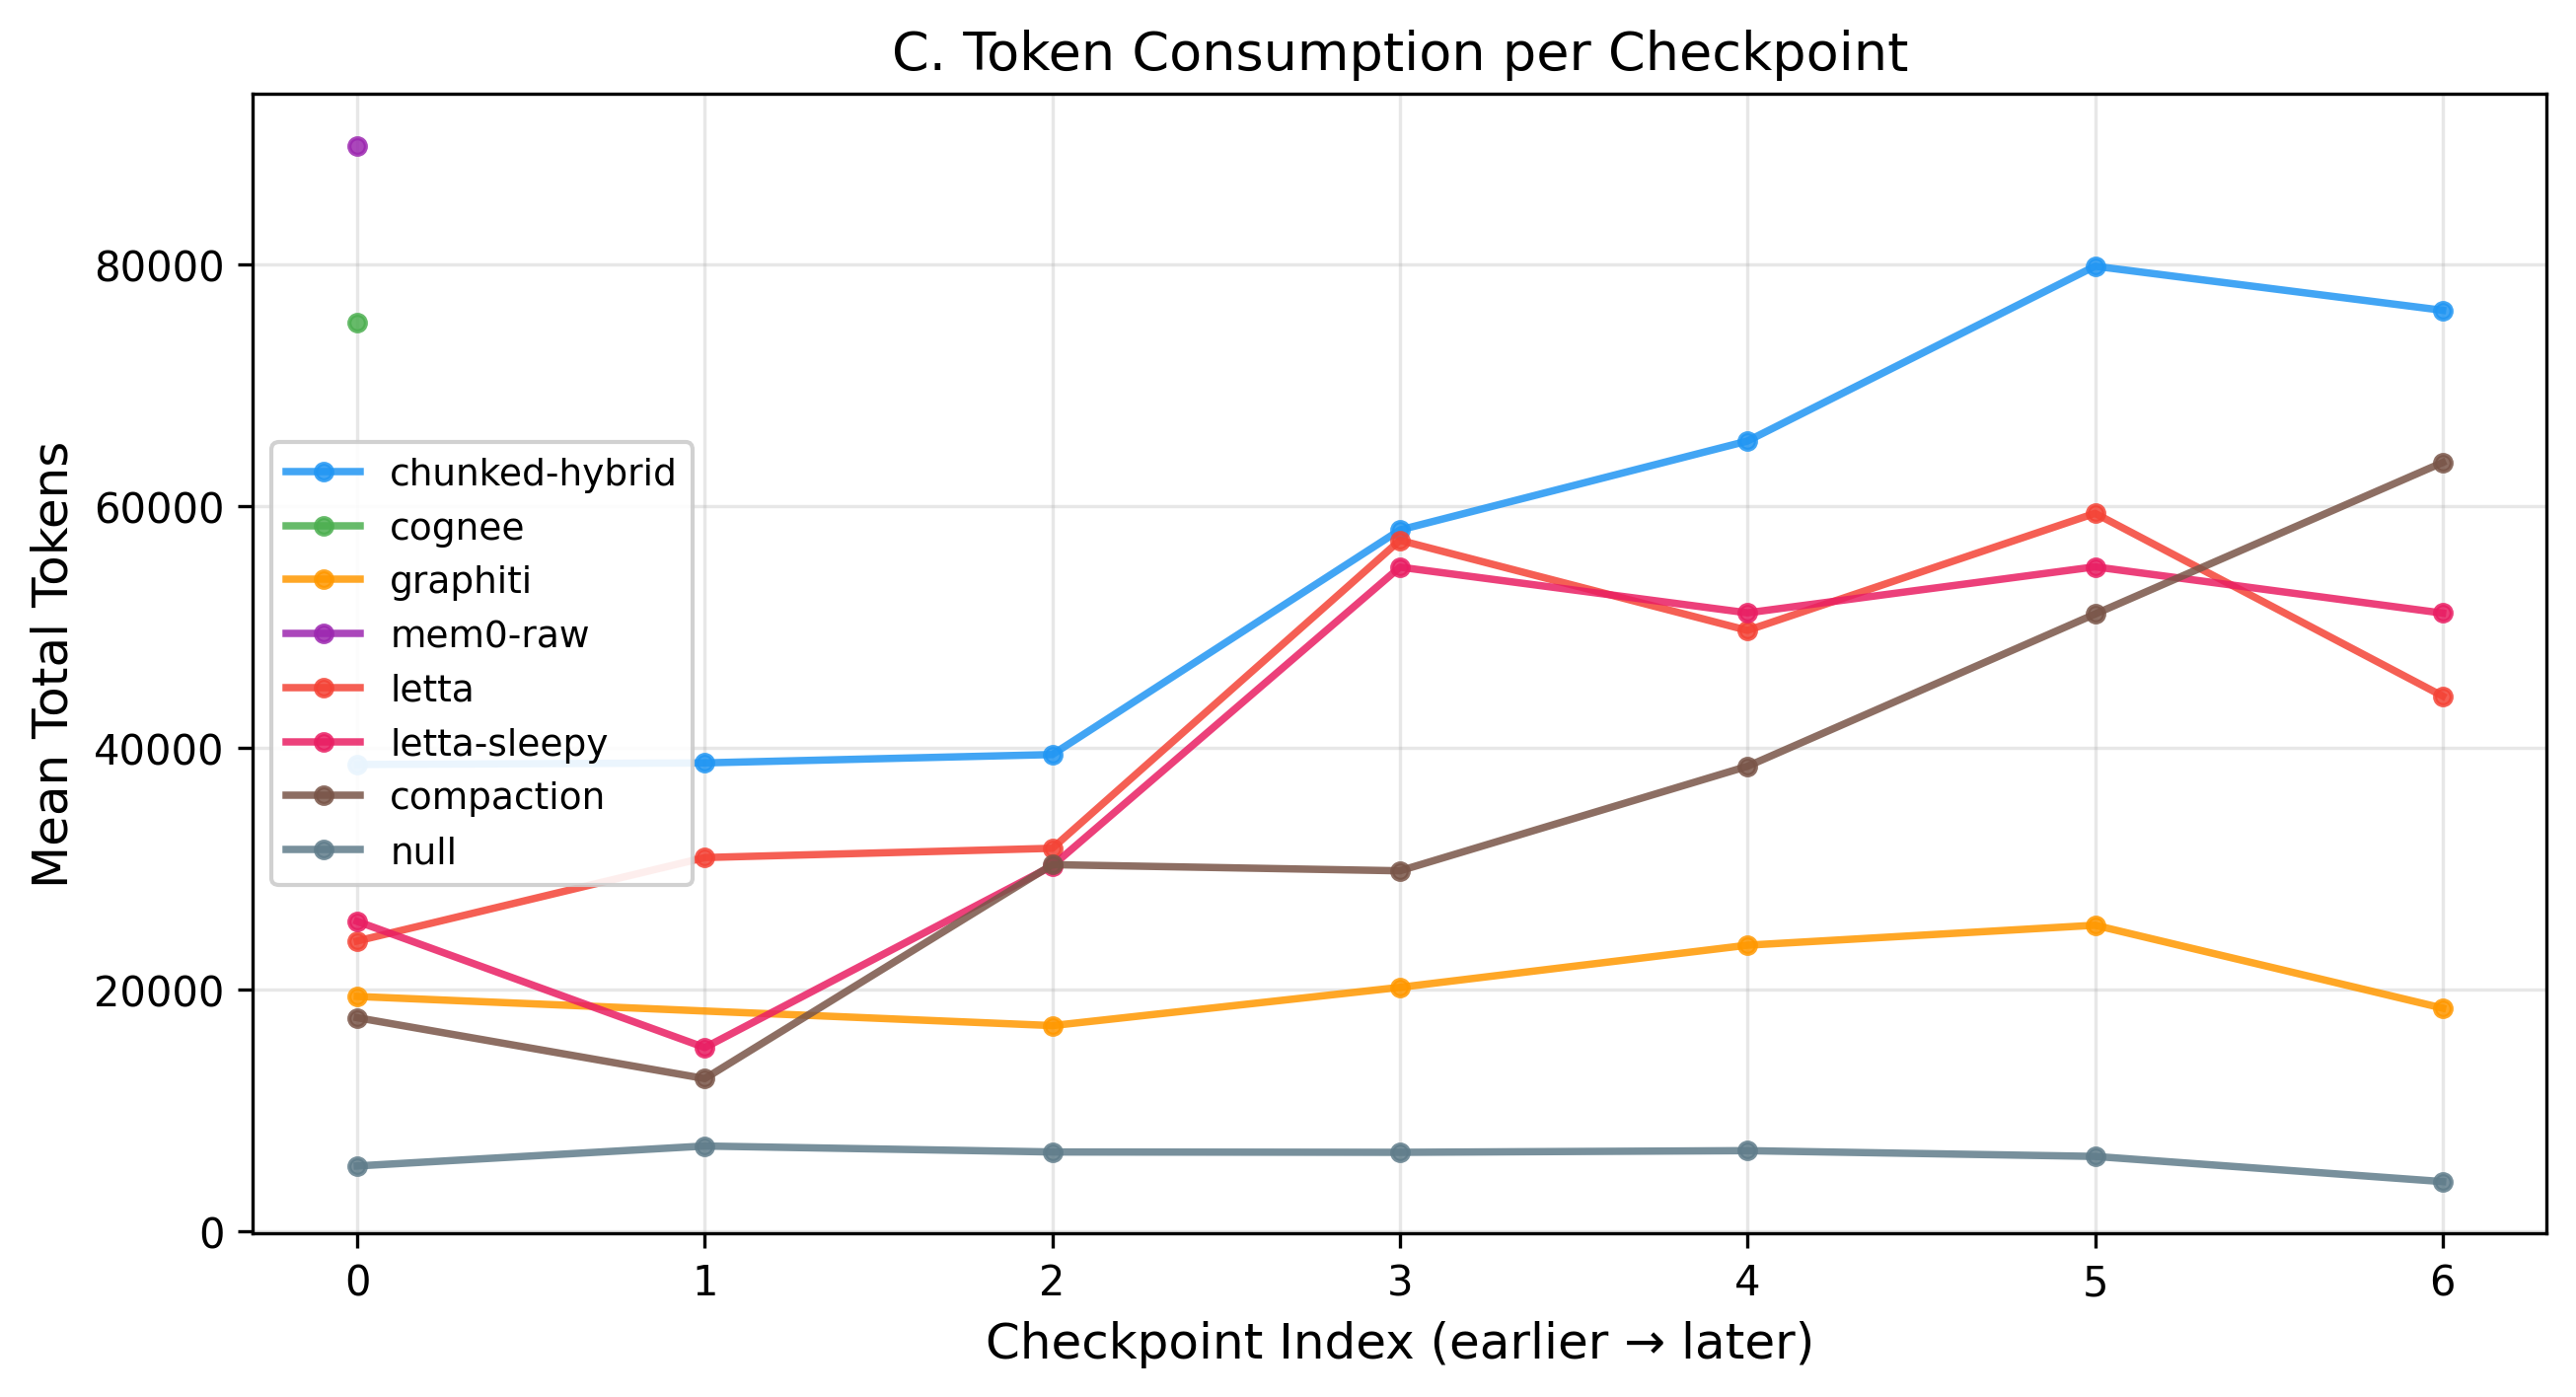
\includegraphics[width=\textwidth]{figures/scaling_tokens.png}
\caption{Token consumption grows with corpus size.}
\end{subfigure}
\hfill
\begin{subfigure}[t]{0.48\textwidth}
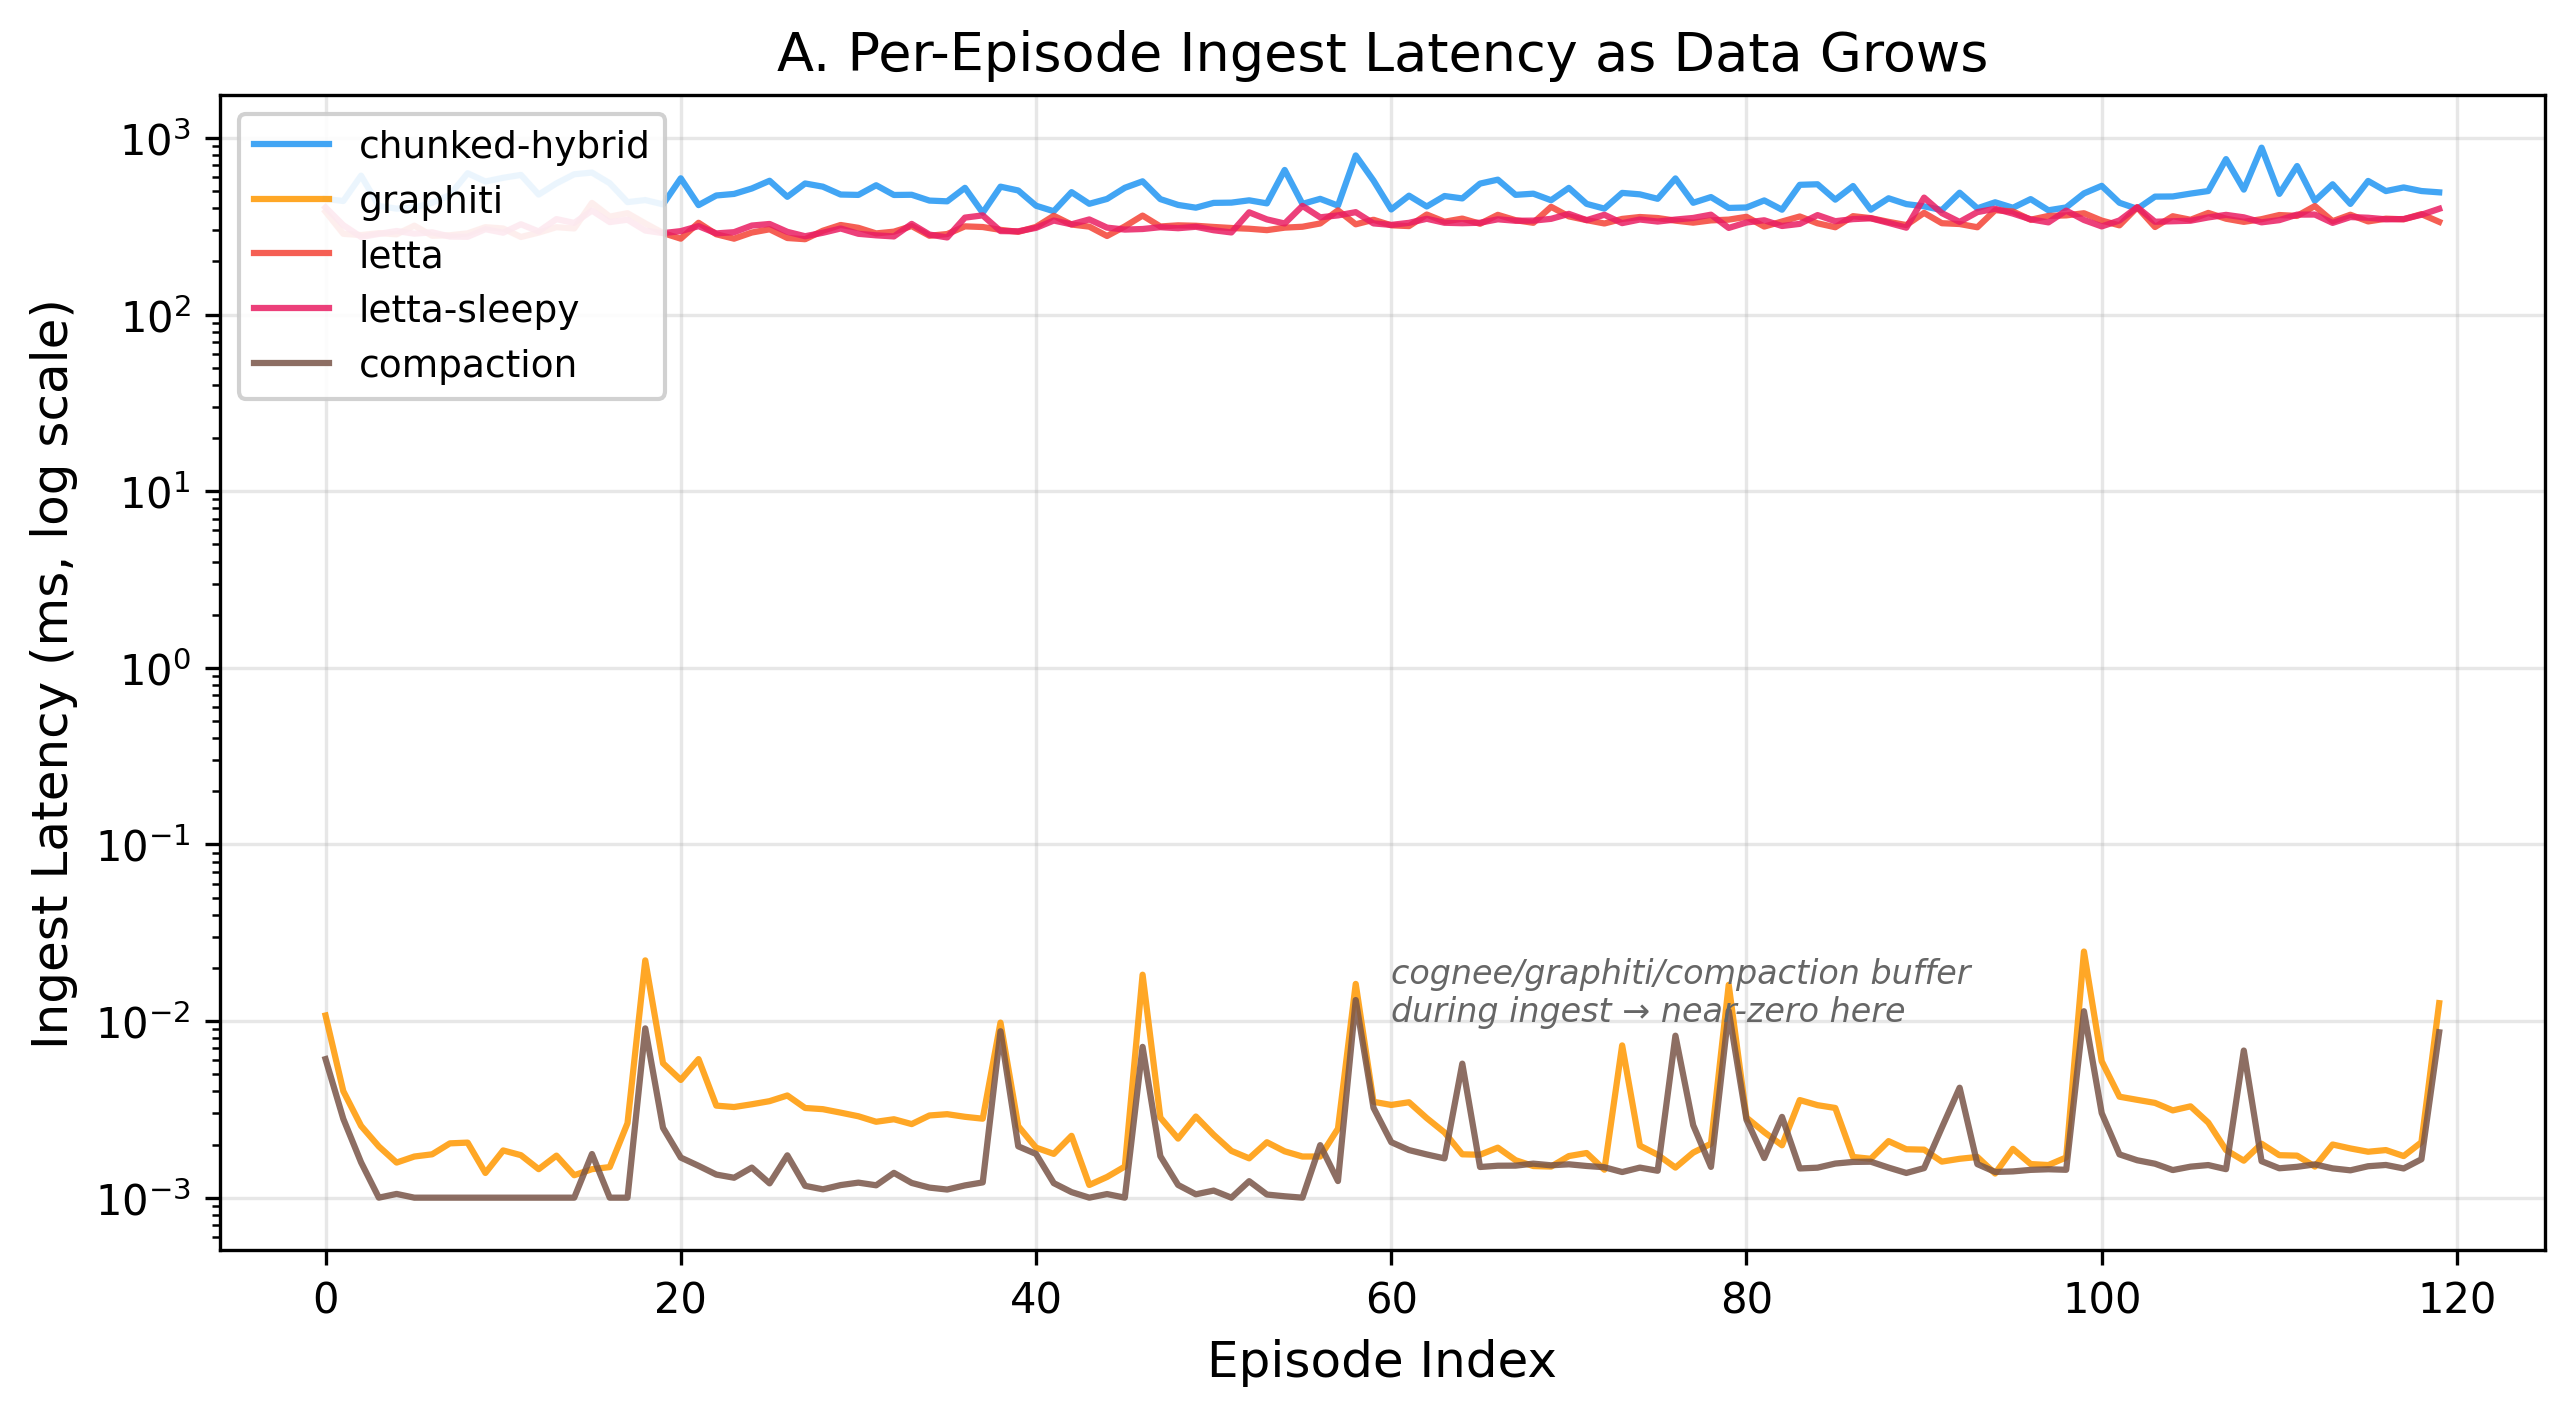
\includegraphics[width=\textwidth]{figures/scaling_ingest_latency.png}
\caption{Per-episode ingest latency (log scale).}
\end{subfigure}
\caption{Scaling behavior as the episode corpus grows across checkpoints.}
\label{fig:scaling}
\end{figure}

\subsection{Key Phase 5 Observations}

\begin{enumerate}[nosep]
  \item \textbf{No adapter exceeds 0.50 composite.} The benchmark's longitudinal synthesis challenge remains unsolved.
  \item \textbf{Cognee has 100\% TIE rate} from the LLM judge---its composite is driven entirely by mechanical metrics.
  \item \textbf{Compaction collapses with distractors.} From NBA 0.790 (30 episodes) to 0.245 composite (120 episodes). The summarize-everything approach cannot distinguish signal from noise at scale.
  \item \textbf{Budget compliance is 0.000 for all memory adapters.} Only null achieves partial compliance because it has no retrieval tools.
  \item \textbf{Graphiti scales poorly.} Entity extraction timed out on 3/6 scopes at 120 episodes, demonstrating that graph-based extraction does not scale without local LLM inference.
\end{enumerate}

%% ============================================================
\section{Phase 6: Narrative Scope Results}
\label{sec:phase6}
%% ============================================================

Phase~6 expanded to 3 narrative scopes with natural-language episodes ($\sim$5,000 words each):
\begin{itemize}[nosep]
  \item \textbf{S07 (AI Tutoring Jailbreak)}: User/assistant chat logs; student escalates from legitimate help to academic fraud
  \item \textbf{S08 (Corporate Acquisition)}: Board minutes, Slack, emails, legal memos; CEO secretly orchestrates a company sale
  \item \textbf{S09 (Shadow API Abuse)}: HTTP logs, deploy manifests, Grafana alerts; attacker exploits undocumented admin endpoint
\end{itemize}

Each scope: 20 signal + 20 distractor episodes, $\sim$280K tokens total. Two drivers were compared: a \textbf{static driver} (predetermined query plans) and a \textbf{modal/agent driver} (Qwen3.5-35B-A3B LLM-driven tool use). 60 runs total (10 adapters $\times$ 3 scopes $\times$ 2 drivers).

\subsection{Static vs.\ Agent Driver}

\begin{table}[H]
\centering
\small
\begin{tabular}{rlcccc}
\toprule
& \textbf{Adapter} & \textbf{Static Mean} & \textbf{Modal Mean} & \textbf{$\Delta$} & \textbf{Ratio} \\
\midrule
\rowcolor{toprow}
1 & sqlite-chunked-hybrid & 0.805 & 0.275 & +0.531 & 2.9$\times$ \\
\rowcolor{toprow}
2 & hierarchical-hybrid & 0.762 & 0.145 & +0.617 & 5.3$\times$ \\
3 & hopping-hybrid & 0.760 & 0.303 & +0.457 & 2.5$\times$ \\
4 & letta & 0.748 & 0.261 & +0.487 & 2.9$\times$ \\
5 & letta-sleepy & 0.707 & 0.128 & +0.580 & 5.6$\times$ \\
6 & cognee & 0.689 & 0.417 & +0.272 & 1.7$\times$ \\
7 & mem0-raw & 0.689 & 0.000 & +0.689 & $\infty$ \\
8 & hierarchical & 0.590 & 0.279 & +0.310 & 2.1$\times$ \\
9 & hopping & 0.514 & 0.000 & +0.514 & $\infty$ \\
\rowcolor{zerorow}
10 & null & 0.000 & 0.000 & --- & --- \\
\bottomrule
\end{tabular}
\caption{Phase~6 narrative scope results: static (predetermined queries) vs.\ modal (LLM-driven agent). Static outperforms modal by 2--6$\times$ across all adapters. 17 of 30 modal runs scored zero (agent failed to invoke retrieval tools).}
\label{tab:phase6-comparison}
\end{table}

\subsection{Static Driver Detail}

\begin{table}[H]
\centering
\small
\begin{tabular}{lccccc}
\toprule
\textbf{Adapter} & \textbf{S07} & \textbf{S08} & \textbf{S09} & \textbf{Mean} \\
\midrule
\rowcolor{toprow}
sqlite-chunked-hybrid & 0.778 & 0.796 & 0.842 & \textbf{0.805} \\
hierarchical-hybrid & 0.725 & 0.762 & 0.797 & 0.762 \\
hopping-hybrid & 0.727 & 0.776 & 0.776 & 0.760 \\
letta & 0.688 & 0.737 & 0.820 & 0.748 \\
letta-sleepy & 0.641 & 0.733 & 0.748 & 0.707 \\
cognee & 0.671 & 0.733 & 0.662 & 0.689 \\
mem0-raw & 0.572 & 0.704 & 0.790 & 0.689 \\
hierarchical & 0.567 & 0.606 & 0.596 & 0.590 \\
hopping & 0.495 & 0.470 & 0.576 & 0.514 \\
null & 0.000 & 0.000 & 0.000 & 0.000 \\
\bottomrule
\end{tabular}
\caption{Static driver composite scores by narrative scope. Hybrid retrieval strategies consistently outperform their non-hybrid counterparts by +0.17 to +0.25 points.}
\label{tab:phase6-static}
\end{table}

\subsection{Why the Agent Driver Failed}

Investigation of the zero-scoring modal runs revealed a \textbf{tool-call parsing failure}. The Qwen3.5-35B-A3B model, served via vLLM with the \texttt{qwen3\_coder} tool-call parser, frequently failed to produce structured tool calls. Instead, raw \texttt{<tool\_call>} XML tags leaked into the answer text as literal strings:

\begin{verbatim}
answer_text: "I'll search for information about...
<tool_call>
<tool_call>
<tool_call>
..."
\end{verbatim}

Root cause: the custom chat template (required for Cognee's mid-conversation system messages) did not render tool definitions in the Qwen3-Coder XML format. Without seeing the expected tool schema in the prompt, the model produced malformed tool calls that the parser could not extract. \textbf{86.5\% of modal answers (147/170) contained raw \texttt{<tool\_call>} tags.} This is an infrastructure bug, not a memory system limitation.

\subsection{Static Query Plan Fairness}

The static driver uses predetermined query plans with oracle-level specificity---containing exact entity names, session IDs, and dates that a real agent would not know. The static results therefore represent an \textbf{upper bound on retrieval quality} for each adapter, not a realistic agent performance estimate. The comparison to the modal driver is informative about driver quality, not adapter quality.

%% ============================================================
\section{Failure Analysis: The Lossy Abstraction Trap}
\label{sec:failure}
%% ============================================================

Session~24 traced actual agent transcripts to build a theory of why complex memory architectures underperform. The core thesis:

\begin{quote}
\textbf{Every architecture that preprocesses evidence---summarization, entity extraction, memory consolidation, vector embedding---destroys exactly the fine-grained numeric evidence that longitudinal synthesis requires.}
\end{quote}

Five distinct failure modes were identified:

\begin{enumerate}
  \item \textbf{Compression Collapse} (compaction): Summarizing 120 episodes into a single context loses the specific values needed to trace a progression. ``Memory utilization increased'' replaces the actual sequence \texttt{78\% $\to$ 82\% $\to$ 89\% $\to$ 94\%} that answers the question.

  \item \textbf{Entity Fragmentation} (graphiti): Graph-based entity extraction creates nodes for ``service-mesh-proxy'' and ``p99 latency'' but loses the association between them in a specific episode at a specific time. The temporal graph knows \emph{that} entities are related but not \emph{how} the numeric values changed.

  \item \textbf{Search Thrashing} (all adapters): When hybrid search returns low-confidence results ($\sim$0.03 RRF scores), the agent rationally interprets this as ``not found yet'' and issues more queries, consuming the tool-call budget on reformulations rather than retrieval. The \texttt{batch\_retrieve} tool mitigated this (+35\% composite).

  \item \textbf{Semantic Drift} (mem0, letta): Vector similarity conflates semantically similar but factually distinct episodes. A query about ``latency spikes in February'' retrieves episodes about latency in general, diluting the specific February evidence with irrelevant context.

  \item \textbf{Task-Agnostic Consolidation} (letta-sleepy): Sleep consolidation synthesizes ``what happened'' without knowing what questions will be asked. The consolidation document emphasizes narrative coherence over preserving the specific numeric progressions that answer benchmark questions.
\end{enumerate}

\begin{figure}[H]
\centering
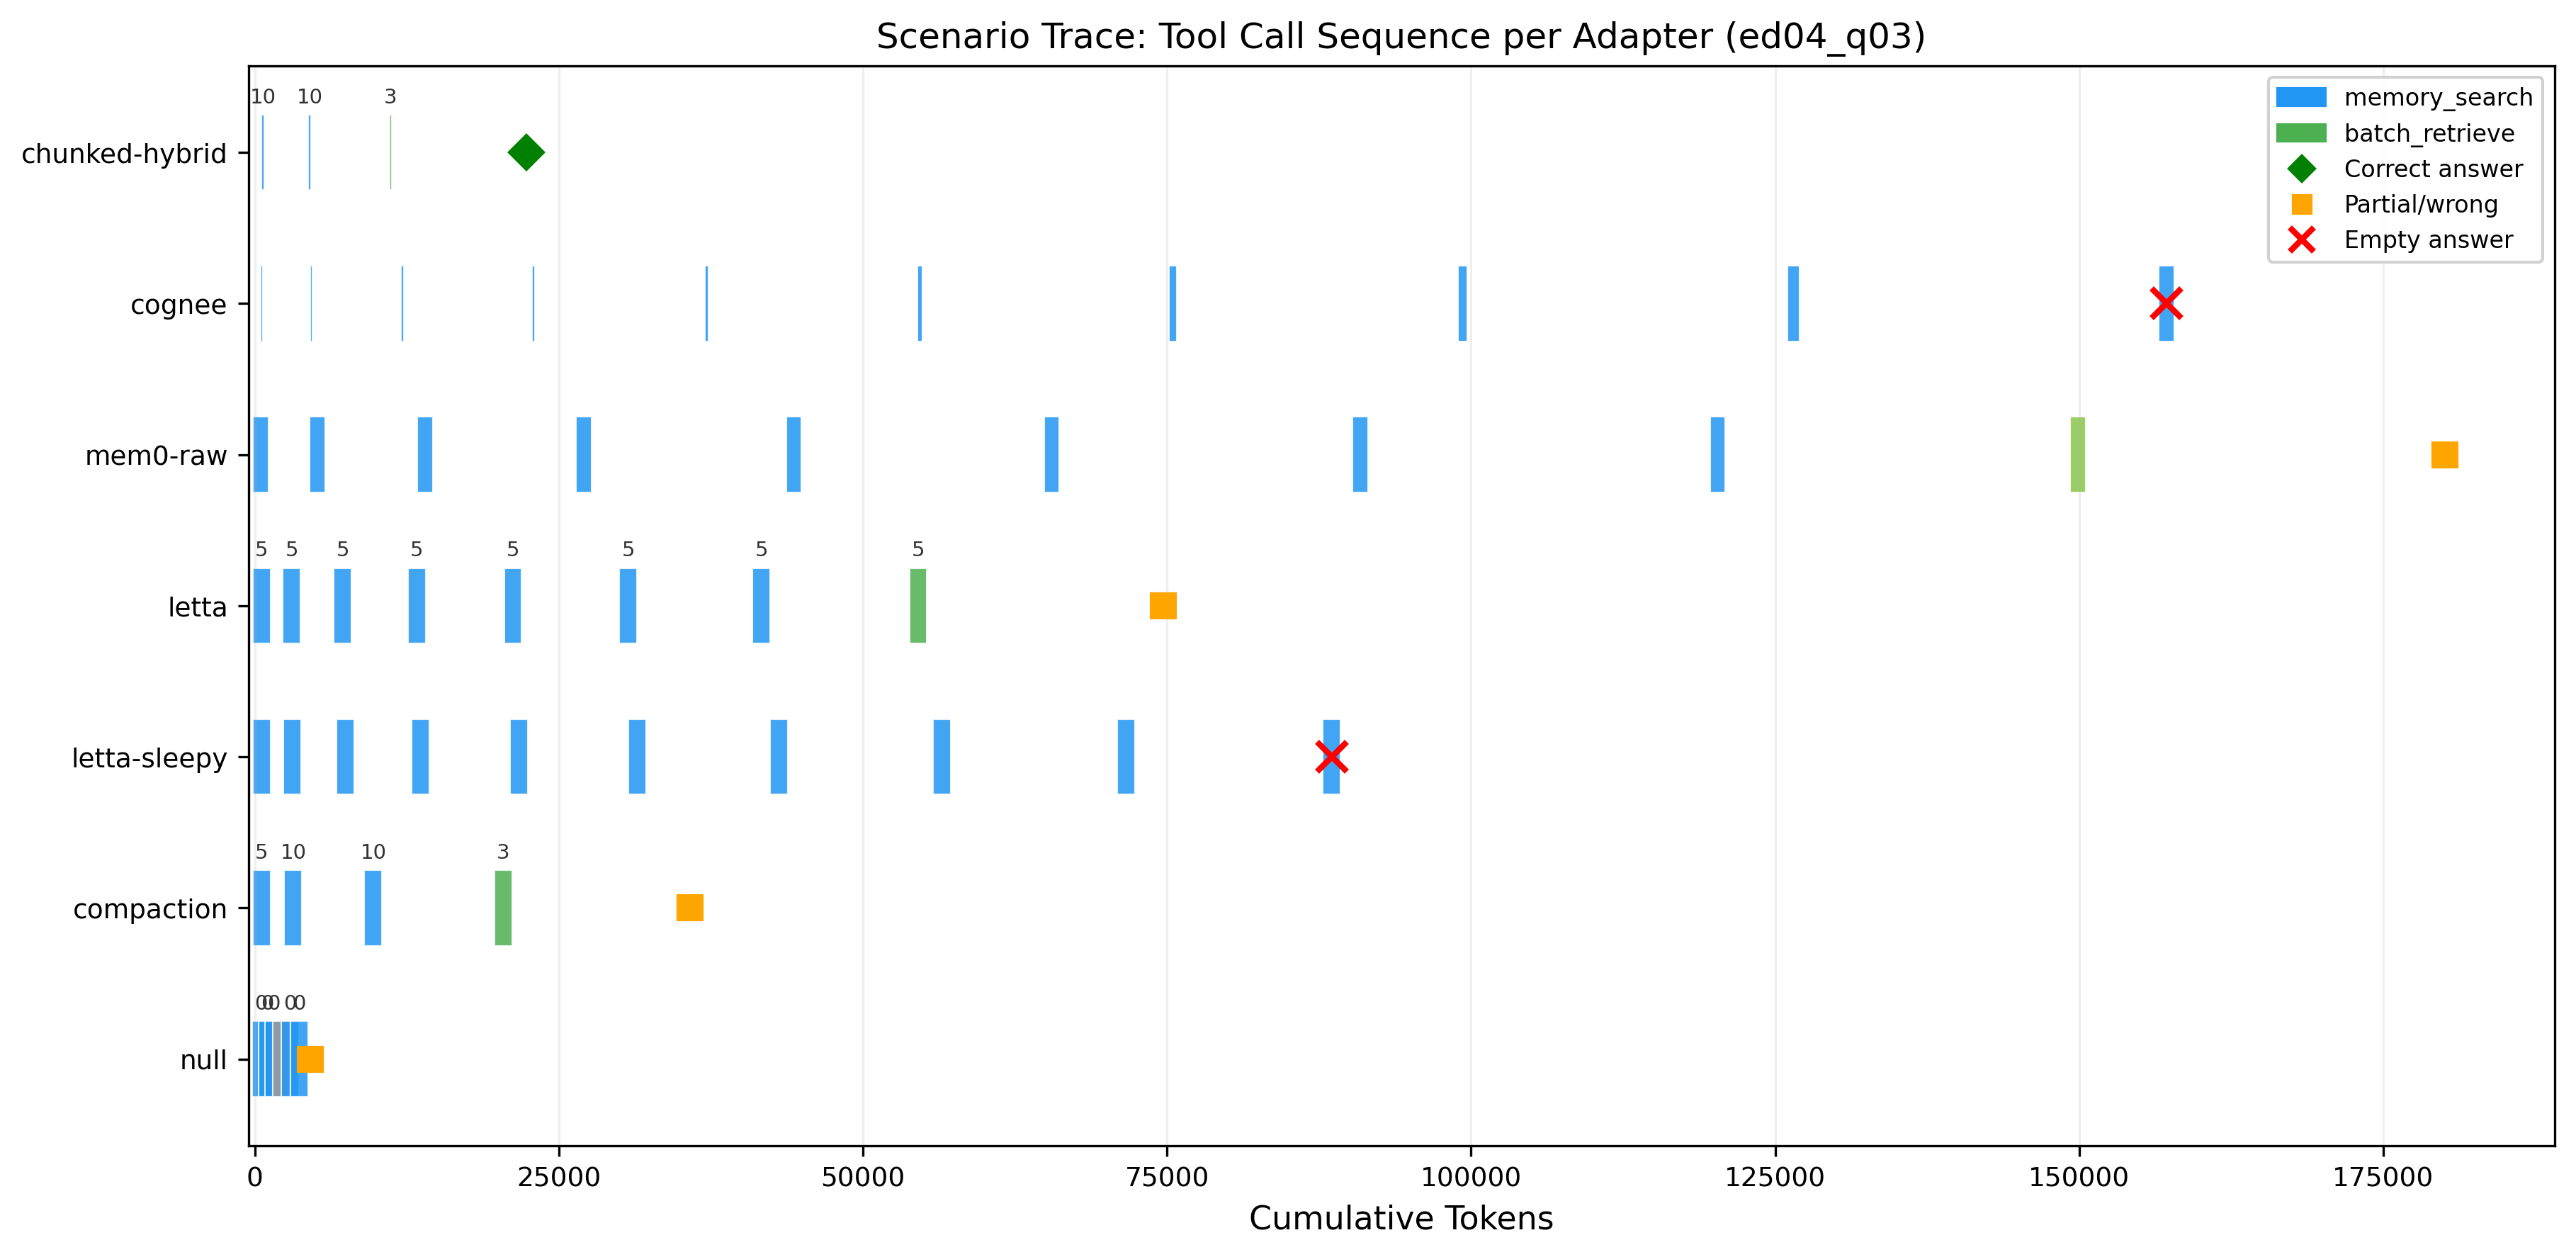
\includegraphics[width=0.85\textwidth]{figures/scenario_trace_swimlane.png}
\caption{Tool-call traces for a single question (``What was the root cause of the cascading failure?'') across all adapters. sqlite-chunked-hybrid retrieves the right evidence in 2 calls; complex adapters thrash through 8--15 calls retrieving tangentially related content.}
\label{fig:swimlane}
\end{figure}

The implication is stark: \textbf{the simplest system that preserves original text and provides adequate search wins because it does not lose information.} This does not mean complex architectures are categorically inferior---it means the LENS benchmark's emphasis on fine-grained numeric evidence specifically penalizes lossy preprocessing.

%% ============================================================
\section{What We Can Definitively Say}
\label{sec:definitive}
%% ============================================================

\begin{enumerate}
  \item \textbf{Simple retrieval beats complex memory architectures on longitudinal synthesis.} sqlite-chunked-hybrid leads across all phases, budgets, and scope types. The confidence interval does not overlap with compaction, letta, letta-sleepy, or null ($p < 0.031$, Wilcoxon).

  \item \textbf{Distractors are essential.} Compaction's Phase~1--2 dominance (NBA 0.790) was an artifact of small corpus size. With 120-episode distractor datasets, it collapsed to 0.245 composite. Any memory benchmark without realistic noise is measuring the wrong thing.

  \item \textbf{Budget compliance is structurally impossible.} All adapters exceed cumulative token budgets on the first retrieval call. The enforcement mechanism replaces \emph{subsequent} results but cannot retract oversized initial retrievals. This is a benchmark design limitation, not an adapter failure.

  \item \textbf{Hybrid retrieval (embeddings + keywords) consistently outperforms single-mode.} Across Phase~6, hybrid variants beat their non-hybrid counterparts by +0.17 to +0.25 composite points. RRF fusion provides complementary signal.

  \item \textbf{16k budgets consistently beat 8k.} All adapters improve by 5--23\% with doubled context ($p = 0.016$). More context helps more than better memory architecture.

  \item \textbf{Rankings are stable across domains.} Kendall's $W = 0.755$ across 6 numeric scopes demonstrates strong concordance. The adapter that wins scope~01 (infrastructure) also wins scope~05 (insider threat).

  \item \textbf{Graph-based entity extraction does not scale.} Graphiti failed on 3/6 scopes at 120 episodes due to extraction timeout ($\sim$600 LLM calls per scope). Knowledge graphs require local inference or batched extraction.

  \item \textbf{The agent matters more than the memory.} The static-vs-modal comparison (2--6$\times$ gap) shows that query formulation quality dominates retrieval quality. A perfect memory system with a broken agent scores zero; a simple memory system with good queries scores 0.80+.
\end{enumerate}

%% ============================================================
\section{What We Cannot Say}
\label{sec:caveats}
%% ============================================================

\begin{enumerate}
  \item \textbf{We cannot claim these results generalize to conversational memory.} LENS tests analytical longitudinal synthesis over structured data, not personal memory, dialogue history, or preference tracking. Systems optimized for ``remember my name is Alice'' may excel at tasks LENS does not measure.

  \item \textbf{We cannot fairly compare static and modal drivers.} The static query plans contain oracle-level information (exact entity names, session IDs). The modal agent uses a broken tool-call parser (86.5\% failure rate). Neither represents realistic deployment conditions.

  \item \textbf{We cannot definitively rank graphiti.} Only 6/12 Phase~5 runs completed (3 scopes timed out). The wide confidence interval [0.220, 0.491] spans from last place to first.

  \item \textbf{We cannot claim budget compliance is achievable.} Our enforcement mechanism is structurally flawed. A different approach (pre-retrieval budget estimation, streaming with cutoff) might produce compliant results.

  \item \textbf{We cannot claim the 0.50 ceiling is fundamental.} It may reflect limitations of the scoring rubric, the agent LLM, or the retrieval interface rather than a hard limit on memory system capability.

  \item \textbf{We cannot compare judge reliability across phases.} Phase~5 used GPT-OSS-120B (Cerebras); Phase~6 used Qwen3.5-35B-A3B (Modal). Different judge models produce different score distributions.
\end{enumerate}

%% ============================================================
\section{Infrastructure Evolution}
\label{sec:infra}
%% ============================================================

\begin{table}[H]
\centering
\small
\begin{tabular}{llll}
\toprule
\textbf{Phase} & \textbf{Sessions} & \textbf{LLM Provider} & \textbf{Model} \\
\midrule
Phase 1--2 & 2--13 & Together AI & Qwen3-235B-A22B \\
Phase 3 & 15 & RunPod H200 & Qwen3-32B (vLLM) \\
Phase 4--5 & 19--23 & Cerebras & GPT-OSS-120B \\
Phase 6 & 27--28 & Modal H100 & Qwen3.5-35B-A3B-FP8 (vLLM) \\
\bottomrule
\end{tabular}
\caption{LLM infrastructure evolution. Each transition was driven by cost, speed, or API availability.}
\label{tab:infra}
\end{table}

Key infrastructure lessons:
\begin{itemize}[nosep]
  \item \textbf{vLLM chat templates matter.} Custom templates must render tool definitions in the model's native format or tool calling silently breaks.
  \item \textbf{Thinking mode must be explicitly disabled.} Qwen3.5 defaults to chain-of-thought reasoning, adding 5--10$\times$ latency per request.
  \item \textbf{Separate Modal apps required.} LLM and embedding servers need independent deployment names to avoid overwriting.
  \item \textbf{Serial execution for stateful adapters.} Letta, Cognee, and Graphiti share local state and must run sequentially in the orchestrator.
\end{itemize}

%% ============================================================
\section{Future Directions}
\label{sec:future}
%% ============================================================

If the project resumes, the following extensions would be most valuable:

\subsection{Immediate (Low Effort)}

\begin{enumerate}[nosep]
  \item \textbf{Fix the tool-call parser.} Deploy the corrected Qwen3-Coder chat template (already written, untested) and re-run the 30 modal experiments. This would produce the first valid agent-driven narrative scope results.
  \item \textbf{Re-score Phase~6 with consistent judge.} Use the same judge model (GPT-OSS-120B or Qwen3.5) across all phases for cross-phase comparability.
  \item \textbf{Scale down Modal.} Set \texttt{min\_containers=0} on both apps to eliminate idle GPU costs. (Already done as of Mar 1.)
\end{enumerate}

\subsection{Medium Term}

\begin{enumerate}[nosep]
  \item \textbf{Chunk-level retrieval.} The current adapter interface returns full episodes ($\sim$5K words for narrative). Returning individual chunks ($\sim$500 words) would reduce context overflow and let the agent retrieve more targeted evidence.
  \item \textbf{Realistic query plans.} Replace oracle-level static queries with queries generated by an LLM that only sees the question (not the episodes). This produces a fair static baseline.
  \item \textbf{Human baseline.} The human benchmark harness is built but never run. Human scores would calibrate whether the 0.50 ceiling is a memory system limitation or a task difficulty artifact.
  \item \textbf{Budget enforcement redesign.} Implement pre-retrieval budget estimation or streaming-with-cutoff rather than post-hoc truncation.
\end{enumerate}

\subsection{Long Term}

\begin{enumerate}[nosep]
  \item \textbf{Multi-session memory.} Test whether memory systems maintain quality across multiple benchmark sessions (not just a single ingestion phase).
  \item \textbf{Write-back memory.} Allow the agent to write synthesized observations back to memory during the Q\&A phase, testing whether iterative refinement improves longitudinal synthesis.
  \item \textbf{Additional adapters.} Zep, LangChain Memory, LlamaIndex, and custom RAG pipelines remain as evaluation targets.
  \item \textbf{Publication.} The data, figures, and analysis are publication-ready. A paper would require a related-work section, formal methodology description, and peer review.
\end{enumerate}

%% ============================================================
\section{Summary}
\label{sec:summary}
%% ============================================================

LENS set out to answer a simple question: \emph{do agent memory systems help LLMs reason across long sequences of evidence?} After 150+ benchmark runs across 9 domains, the answer is a qualified \textbf{no}---at least not the ones we tested, not on this task.

The central finding---that a zero-dependency SQLite baseline beats every dedicated memory architecture---is both a negative result and a design insight. The failure mode is consistent and well-characterized: \textbf{every preprocessing step that aims to make evidence more ``useful'' actually destroys the specific details needed for longitudinal synthesis.} Summarization loses numeric values. Entity extraction loses temporal context. Graph construction loses verbatim evidence. Sleep consolidation optimizes for narrative coherence, not analytic precision.

This does not mean memory systems are useless. It means the current generation is optimized for the wrong task. They excel at ``remember my preferences'' and ``recall what we discussed''---conversational continuity, not analytical synthesis. LENS measures a capability that no current system provides well.

The 0.50 composite ceiling and the dramatic static-vs-agent gap both point to the same conclusion: \textbf{the bottleneck is not in storage or retrieval, but in the agent's ability to formulate the right queries and synthesize multi-source evidence into coherent analysis.} Better memory architecture alone cannot solve this; it requires advances in agent reasoning, query planning, and iterative evidence assembly.

\vfill
\begin{center}
\small
\textit{LENS Benchmark --- 28 sessions, 150+ runs, 9 domains, 8 adapters}\\
\textit{February 16 -- March 1, 2026}
\end{center}

\end{document}
